\section{Git Model}
\label{apx:git}

\begin{figure}[h!]
  \caption{Git branching model}
  \centering
    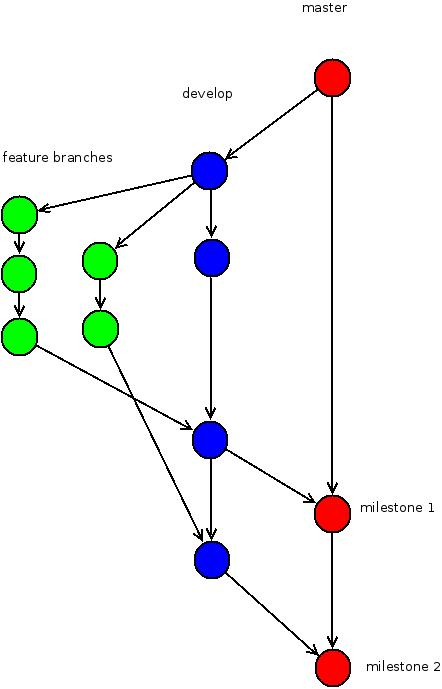
\includegraphics[width=0.8\textwidth]{gitbranch.jpg}
\end{figure}

\begin{itemize}
    \item The master branch was treated as sacred, only being updated after
    a milestone code was completed.
    \item The main working branch was the develop branch. New features were
    branched off of here.
    \item New features were merged back into develop when completed and the
    feature branch deleted.
    \item The master was tagged at each milestone.
\end{itemize}

This branching model was based on
\url{http://nvie.com/posts/a-successful-git-branching-model/}.

